\documentclass{zjureport}
\usepackage{hyperref}
% =============================================
% Part 0 Edit the info
% =============================================

\major{机械制造及自动化}
\name{刘源}
\title{实验报告}
\stuida{201828013919034}
\college{光电学院}
\date{\zhtoday}
\lab{寝室}
\course{计算机网络}
\instructor{谢高岗}
\expname{广播网络实验}
\exptype{设计实验}

\begin{document}
% =============================================
% Part 1 Header
% =============================================
\makecover
\makeheader

% =============================================
% Part 2 Main document
% =============================================

\section{实验要求}
  本实验要求学生在已有代码基础上,实现节点广播的broadcast\_packet函数,验证广播网络能够正常运行,验证广播网络的效率,验证环形拓扑下会产生数据报回路。

\section{实验内容和步骤}
  \subsection{实现节点广播的broadcast\_packet函数}
  \subsection{验证广播网络正常运行}

      \begin{enumerate}
          \item 运行网络拓扑(three\_nodes\_bw.py)
          \item 在b1交换机节点上编译运行hub程序
          \item 从h1(10.0.0.1) Ping h2(10.0.0.2)和h3(10.0.0.3),能够ping通
          \item 从h2(10.0.0.2) Ping h1(10.0.0.1)和h3(10.0.0.3),能够ping通
          \item 从h3(10.0.0.3) Ping h1(10.0.0.1)和h2(10.0.0.2),能够ping通
      \end{enumerate}

  \subsection{验证广播网络的效率}

      \begin{enumerate}
          \item 运行网络拓扑(three\_nodes\_bw.py)
          \item 在b1上运行hub程序
          \item 在h2和h3上执行 iperf -s 命令
          \item 在h1上依次执行 iperf -c 10.0.0.2 -t 30 和 iperf -c 10.0.0.3 -t 30 命令,得到实验结果
          \item 在h1上执行iperf -s命令
          \item 在h2和h3上分别执行 iperf -c 10.0.0.1 -t 30 命令,得到实验结果
      \end{enumerate}

  \subsection{验证环形拓扑下会产生回路}
    \begin{enumerate}
      \item 运行网络拓扑(ring\_topo.py)
      \item 在b1、b2、b3上运行hub程序
      \item 在h2(10.0.0.2)上运行wireshark软件并监听数据报
      \item 从h1(10.0.0.1) Ping h2(10.0.0.2),分析wireshark数据,得到实验结果
    \end{enumerate}

\section{主要仪器设备}
  计算机,Mininet 软件,Wireshark 软件

\section{实验过程}
  \subsection{安装mininet与wireshark软件}
     在Ubuntu下输入sudo apt install mininet 与 sudo apt install build-essential xterm wireshark ethtool iperf traceroute iptables arptables命令进行软件安装,安装完成后,运行sudo mn验证mininet是否正确安装,验证结果如图~\ref{fig:install} 所示。
           \begin{figure}[!htbp]
               \centering
               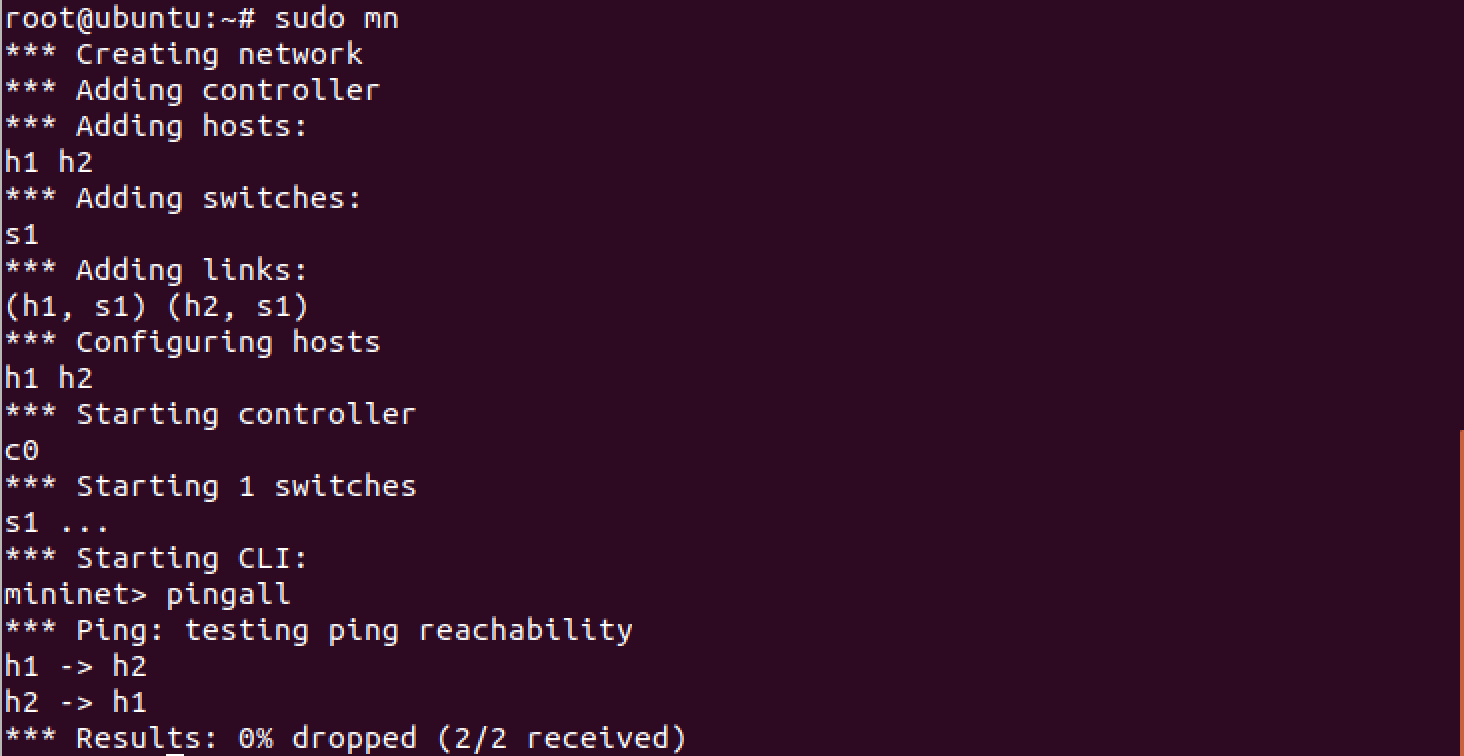
\includegraphics[width=0.7\linewidth]{figures/02.jpg}
               \caption{mininet安装成功}
               \label{fig:install}
           \end{figure}

  \subsection{编写broadcast\_packet函数}
      \lstinputlisting[language=C]{code/broadcast_packet.c}

  \subsection{依步骤完成实验内容}

  \section{实验结果与分析}
  \subsection{验证广播网络正常运行}
      \begin{enumerate}
          \item 运行broadcast\_packet.py生成的网络如图~\ref{fig:03} 所示。
                \begin{figure}[!htbp]
                    \centering
                    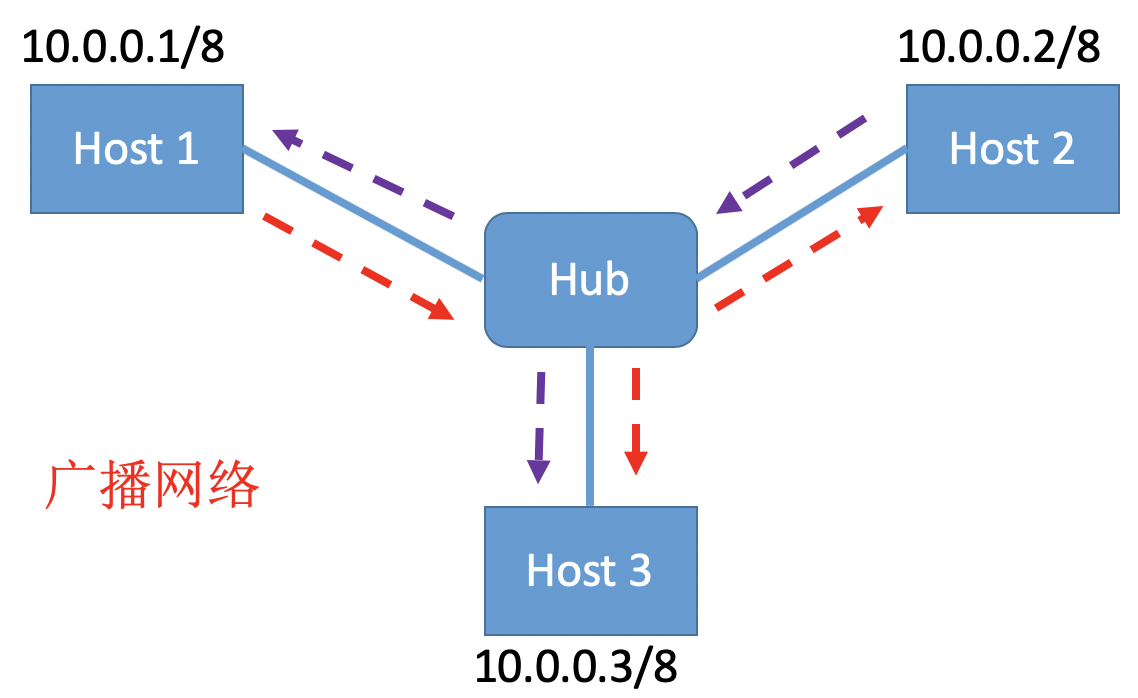
\includegraphics[width=0.7\linewidth]{figures/03.jpg}
                    \caption{broadcast\_packet.py生成的网络}
                    \label{fig:03}
                \end{figure}

          \item 编译并在b1上运行hub程序,程序运行结果如图~\ref{fig:04}所示。
            \begin{figure}[!htbp]
              \centering
              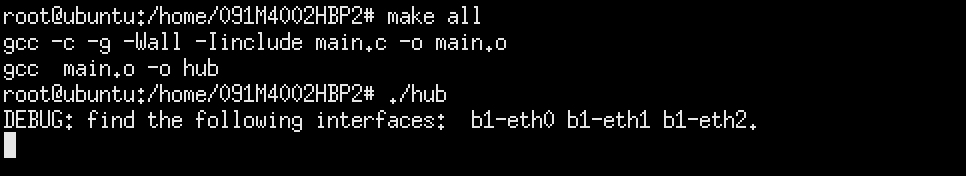
\includegraphics[width=0.7\linewidth]{figures/04.jpg}
              \caption{hub程序运行结果}
              \label{fig:04}
            \end{figure}

          \item 从h1(10.0.0.1) Ping h2(10.0.0.2)和 h3(10.0.0.3),结果如图~\ref{fig:05}所示,能够Ping通。
            \begin{figure}[!htbp]
              \centering
              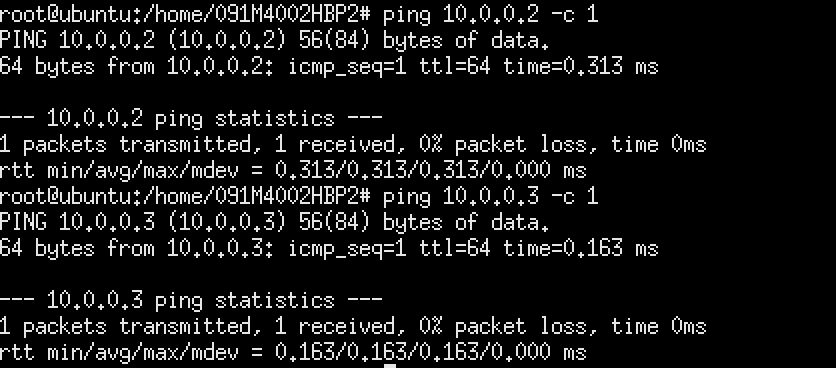
\includegraphics[width=0.7\linewidth]{figures/05.jpg}
              \caption{从h1 Ping h2和h3结果}
              \label{fig:05}
            \end{figure}

          \item 从h2(10.0.0.2) Ping h1(10.0.0.1)和h3(10.0.0.3),结果如图~\ref{fig:06}所示,能够ping通。
            \begin{figure}[!htbp]
              \centering
              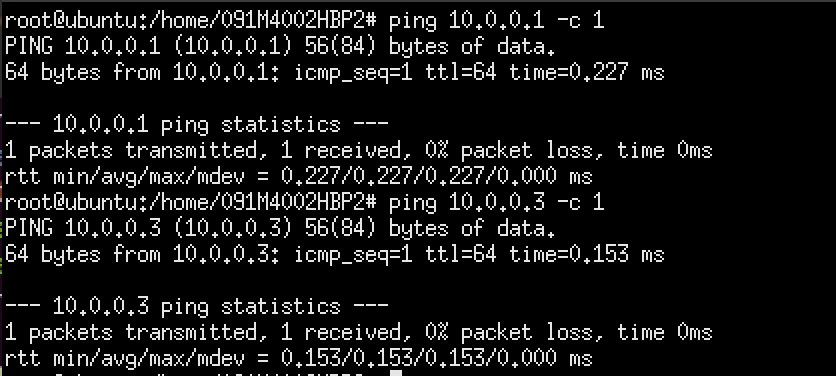
\includegraphics[width=0.7\linewidth]{figures/06.jpg}
              \caption{从h2 Ping h1和h3结果}
              \label{fig:06}
            \end{figure}

            \item 从h3(10.0.0.3) Ping h1(10.0.0.1)和h2(10.0.0.2),结果如图~\ref{fig:07}所示,能够ping通。
              \begin{figure}[!htbp]
                \centering
                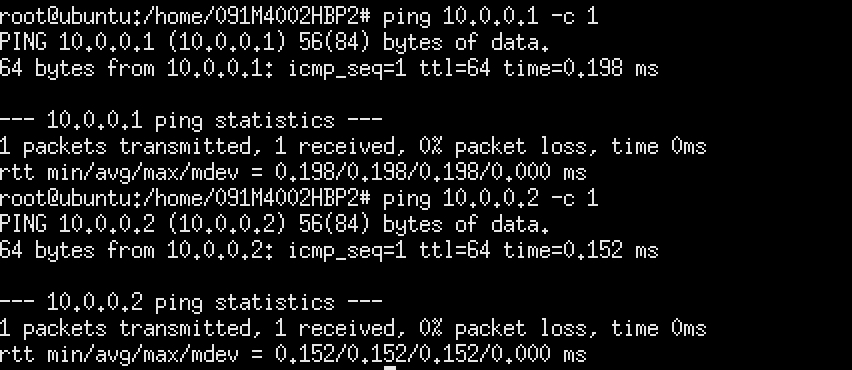
\includegraphics[width=0.7\linewidth]{figures/07.jpg}
                \caption{从h3 Ping h1和h2结果}
                \label{fig:07}
              \end{figure}

          \item 广播网络各节点能相互ping通,证明broadcast\_packet函数能够完成实验所需功能,实验成功。

      \end{enumerate}

  \subsection{验证广播网络的效率}
  \begin{enumerate}
      \item 运行broadcast\_packet.py
      \item 在b1节点上运行hub程序
      \item 依次在h2和h3上执行 iperf -s 命令,\ref{label:exeresult}执行后h2 iperf程序结果如图~\ref{fig:08}所示。
        \begin{figure}[!htbp]
          \centering
          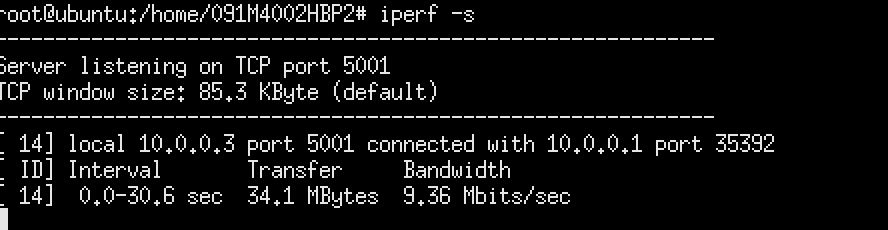
\includegraphics[width=0.7\linewidth]{figures/08.jpg}
          \caption{h2和h3执行iperf server测试结果}
          \label{fig:08}
        \end{figure}

      \item \label{label:exeresult} 在h1上依次执行 iperf -c 10.0.0.2 -t 30 和 iperf -c 10.0.0.3 -t 30 命令,结果如图~\ref{fig:09}所示。
        \begin{figure}[!htbp]
          \centering
          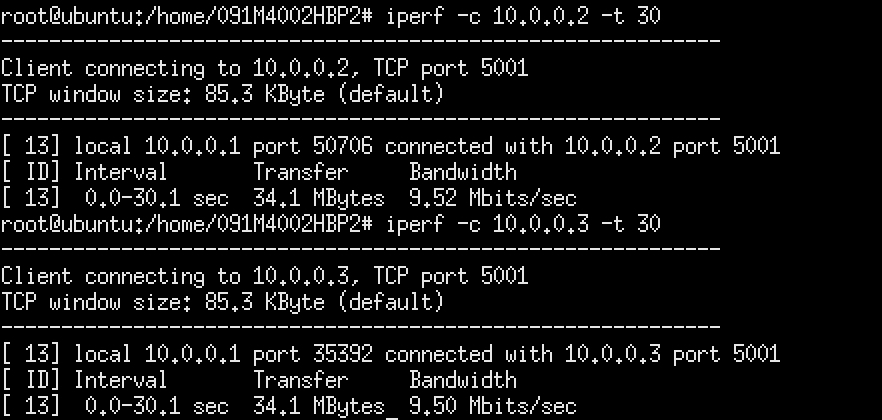
\includegraphics[width=0.7\linewidth]{figures/09.jpg}
          \caption{h1执行iperf client测试结果}
          \label{fig:09}
        \end{figure}

      \item 在h1上执行iperf -s命令,\ref{label:exe2result}执行后h1 iperf程序结果如图~\ref{fig:10}所示。
        \begin{figure}[!htbp]
          \centering
          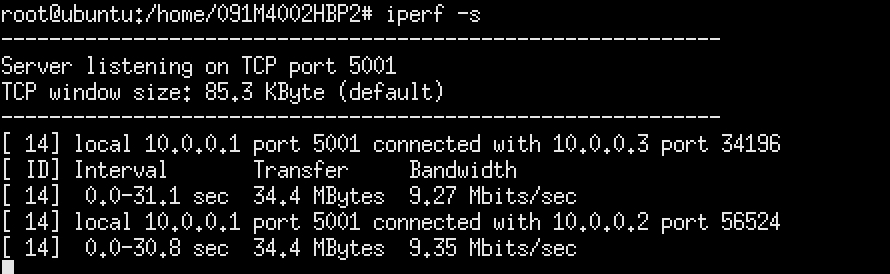
\includegraphics[width=0.7\linewidth]{figures/10.jpg}
          \caption{h1执行iperf server测试结果}
          \label{fig:10}
        \end{figure}

      \item \label{label:exe2result} 在h2和h3上分别执行 iperf -c 10.0.0.1 -t 30 和 iperf -c 10.0.0.1 -t 30 命令,h2的运行结果如图~\ref{fig:11}所示,h3的运行结果如图~\ref{fig:12}所示。
        \begin{figure}[!htbp]
          \centering
          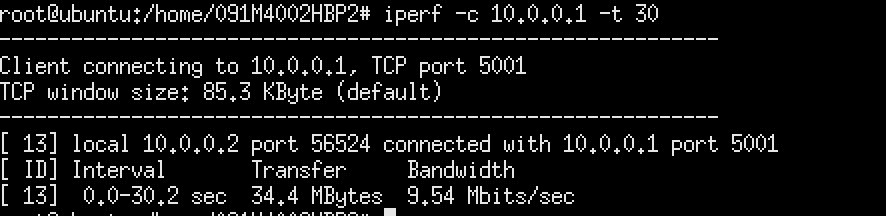
\includegraphics[width=0.7\linewidth]{figures/11.jpg}
          \caption{h2执行iperf client测试结果}
          \label{fig:11}
        \end{figure}

        \begin{figure}[!htbp]
          \centering
          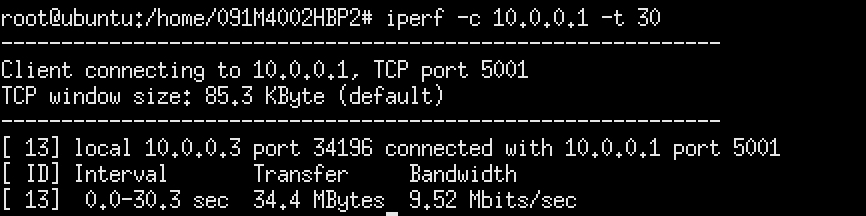
\includegraphics[width=0.7\linewidth]{figures/12.jpg}
          \caption{h3执行iperf client测试结果}
          \label{fig:12}
        \end{figure}

    \item 以上实验结果表明,h2与hub以及h3与hub之间的链路带宽和脚本中所设置的10Mb/s基本一致,实验成功。

  \end{enumerate}

  \subsection{验证环形拓扑下会产生回路}
  \begin{enumerate}
    \item 运行网络拓扑(ring\_topo.py),产生的网络结构如图~\ref{fig:13}所示。
      \begin{figure}[!htbp]
        \centering
        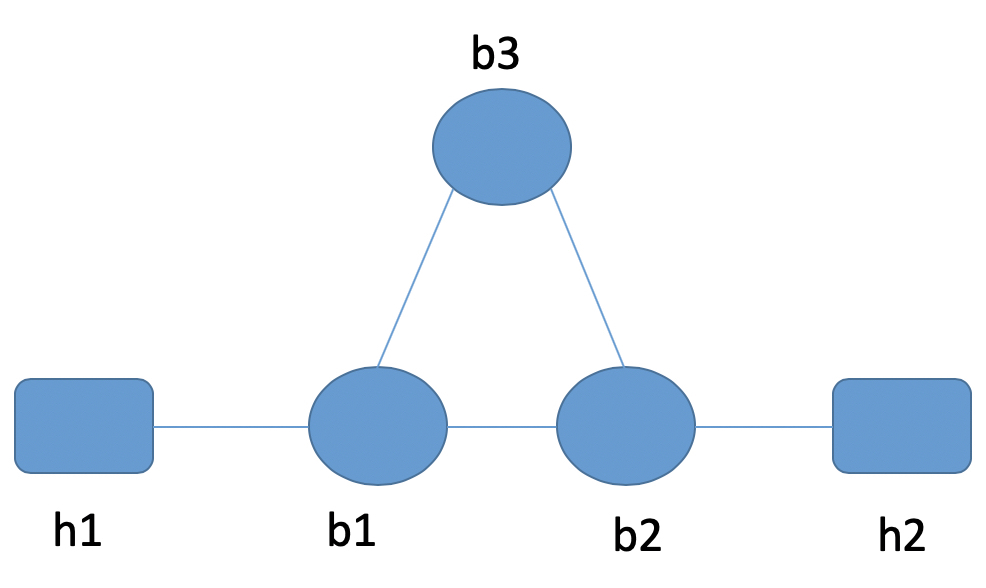
\includegraphics[width=0.7\linewidth]{figures/13.jpg}
        \caption{ring\_topo.py运行结果}
        \label{fig:13}
      \end{figure}

    \item 在b1、b2、b3上运行hub程序。

    \item 在h2(10.0.0.2)上运行wireshark软件并监听数据报,在\ref{label:exe3result}执行后结果如图~\ref{fig:14}所示。

    \item \label{label:exe3result} 从h1(10.0.0.1) Ping h2(10.0.0.2),分析wireshark数据,由图~\ref{fig:14}可知,环路中有数据包在不断的转发,实验成功。
      \begin{figure}[!htbp]
        \centering
        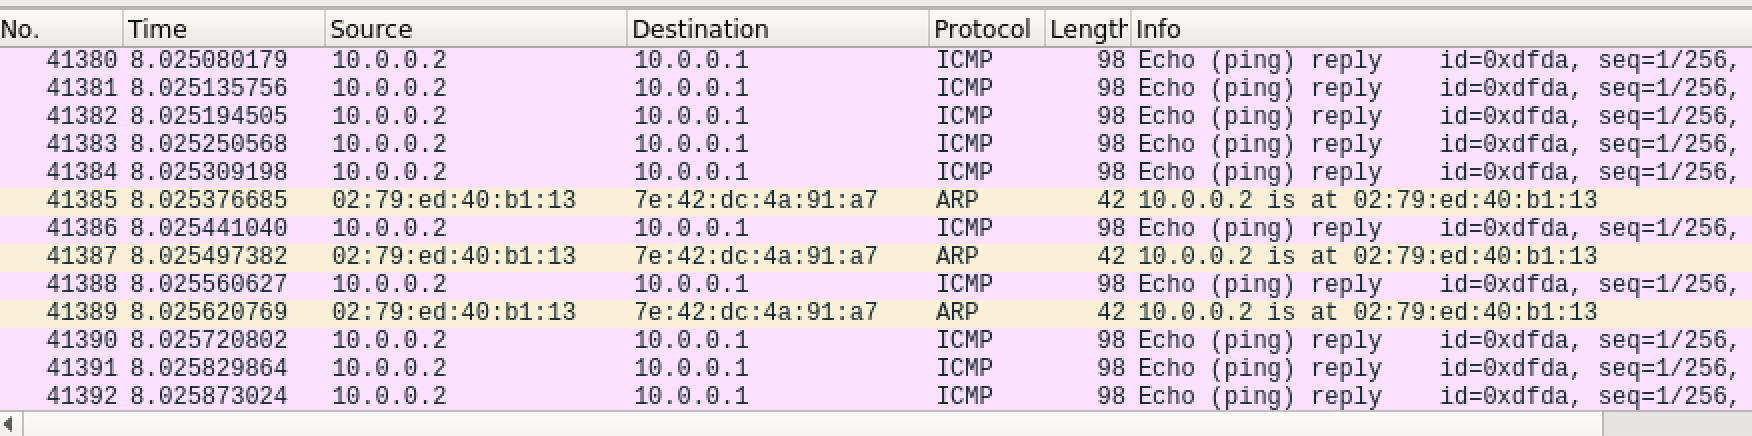
\includegraphics[width=0.9\linewidth]{figures/14.jpg}
        \caption{h2上wireshark程序抓包的部分结果}
        \label{fig:14}
      \end{figure}
  \end{enumerate}

\end{document}
